\subsection{Segmentation}
%recuperation d'un objet dans l'environnemnt -> interaction utilisateur
%dire que la création d'une base de connaissance est plus utile que pour le corps humain
La première étape lors de notre projet va être de segmenter les images que nous recevons de 
notre caméra. Les informations contenues dans une image 3D sont nombreuses et nous devons
déterminer les éléments important pour nos traitements. Dans notre scène,
nous avons besoin des objets proches ou du corps de la personne en face de la caméra, mais 
l'environnement autour des ces objets clés n'est pas important et doit être supprimer pour
gagner du temps lors de nos traitements en supprimant de l'information à traiter.
Une second segmentation est nécessaire pour le traitement du corps humain. Pour cette étape du projet,
nous devons segmenter le corps en plusieurs partie pour pouvoir par la suite les reconnaitres. Si cette
seconde segmentation n'est pas réalisé il ne nous sera pas possible de reconnaître les mains ou encore
la tête si nous ne savons délimité les parties du corps.  

\begin{figure}[!h]
  \begin{center}
    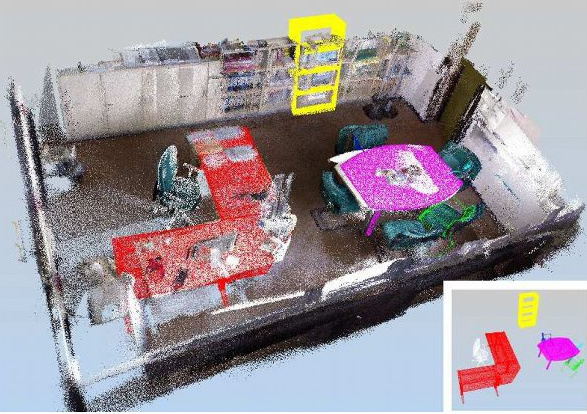
\includegraphics[width=8cm]{image/segmentation.png}
    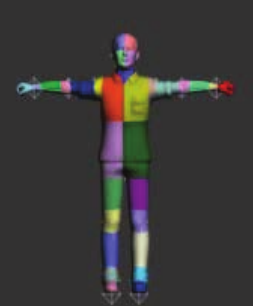
\includegraphics[width=5cm]{image/bodySegmentation.png}
    \caption{Exemple de segmentation recherché pour une pièce intérieur et pour le corps humain}
  \end{center}
\end{figure}
 
\subsubsection{Scène intérieur}
De nombreux travaux ont été réalisé dans la segmentation d'image 2D avant que les caméras 3D ne soit
ouvert au grand public. Les premières méthode de segmentation reposaient sur la détection de contour
comme pour la méthode de P. Arbelaez et al\cite{2DSegmentation1}. Leur méthode repose sur le détecteur
de contour gPb qui est composé de d'un seuillage sur la luminance et sur la couleur et d'une détection
de texture. La fermeture des contours se fait ensuite en utilisant les superpixels. D'autres méthodes
2D utilise un simple seuillage en utilisant par exemple la méthode de N. Otsu\cite{Otsu} pour binariser
l'image et ainsi la segmenter.\\

%peut etre que l on peut rajouter des publi utilisant la depthmap
%voir si on sépare la depthmap et le nuage de point
Avec l'arrivé des caméras 3D de nombreuses recherche ont été effectué sur la segmentation d'image à partir
des information extraite de ce type de caméra. S.A.A Shah et al\cite{3DSegmentation1} utilisent les informations
de l'image de profondeur afin de calculer un vecteur sur chaque pixel. En applicant un seuillage sur la différence
des vecteurs ils obtiennent une segmentation de l'environnement qui leur permet de détecter des objets dans une pièce.
Il est possible à partir de l'image de profondeur de créer un nuage de point, ce qui permet d'obtenir les 
coordonnées 3D des points présents dans l'image de profondeur. Les informations qu'il est possible d'extraire
d'un nuage de point sont différentes et des méthodes de segmentation se sont développé autour de ces informations.\\

T. Rabbani et al\cite{pointCloudSegmentation} utilise les informations obtenus dans un nuage de point afin 
de calculer les normales de chaque point. Ils segmente ensuite l'image en comparant les normales et en appliquant
un seuillage sur cette comparaison. Si l'angle formé par les normales de deux points est super au seuil alors
les points appartiennent à deux régions différentes.\\

Nous pouvons voir que les méthodes cité précédemment sont efficace pour segmenter une scène comportant des objets,
mais elles ne sont pas applicable à un corps humain. Le principal défaut de ces méthodes pour le corps humain est 
que celui-ci est trop lisse. La différence entre les normales ou entre les vecteurs de pixel n'est pas assez important
et est trop instable pour que cela marche sur le corps humain.

\subsubsection{Corps humain}
La segmentation du corps humain est un sujet très complexe, car contrairement au objet celui-ci bouge et adopte
des postures différentes. La méthode la plus souvent utilisé pour résoudre cette problématique est de déterminer
la posture de l'utilisateur et lorsque cette posture est connu il est facile de déterminer les différentes partie
du corps. Ces méthodes nécessitent d'avoir une base de connaissance contenant de nombreuses postures qui doivent
être segmenter et labelisé avec les différentes parties du corps. J. Shotton et al\cite{kinectSegmentation} ont
d'abord créé une base d'apprentissage en calculant un descripteur\footnote{Voir \ref{descriptor}}
et une technique d'apprentissage automatique appelé forêt d'arbres décisionnels\cite{randomDecisionForest}. 
Lorsque l'utilisateur bouge, le descripteur utilisé précédemment est recalculé sur l'image courante et le résultat 
est comparé au posture de la base d'apprentissage. La posture ayant une valeur proche du résultat calculé précédemment 
est la posture de l'utilisateur. De nombreuses méthode utilise cette solution, mais elle modifie le descripteur
utilisé et la technique d'apprentissage automatique comme nous le verrons dans la suite de ce rapport.

\subsection{Reconnaissance d'objets}
La reconnaissance d'objet est un sujet assez vaste dans le monde de l'imagerie et il existe de nombreuses
méthodes dans le domaine que ce soit pour des images 2D ou 3D. Dans le cas d'image 3D la méthode la plus utilisé
est le calcul de descripteur, ce qui correspond à un ensemble de caractèristiques représentant un objet spécifique.

\subsubsection{Descripteur}
\label{descriptor}
Le nombre de descripteur qui existe dans le domaine de l'image 3D est assez important c'est pourquoi pour ce rapport,
nous allons nous contenter de décrire seulement les plus utilisées. Le descripteur D2\cite{D2} est un des outils de 
comparaison de forme 3D les plus simple à réaliser. Il se repose sur le calcul de la distance euclidienne entre 
chaque point du modèle 3D. L'ensemble de ces distances permet de créer un histogramme 1D et de comparer ces histogramme
afin de reconnaître un objet. Ce descripteur fournit de bon résultat lorsque les objets à reconnaître sont très 
différents.\\

Le descripteur PFH\cite{PFH} est un outil permettant de calculer la courbure moyenne d'un voisinage de point en utilisant
un histogramme multi-dimensionnel. Le calcul de la courbure et le fait que ce soit une généralisation permet d'être invariant 
en translation et en rotation, et permet également d'être moins sensible au bruit présent dans le nuage de point. Le voisinage 
dépend de la distance des points avec le point centrale et il ne peut exceder un certain nombre de voisin (voir Fig. \ref{fig:pfhNeighborhood}).
\begin{figure}[!h]
  \begin{center}
    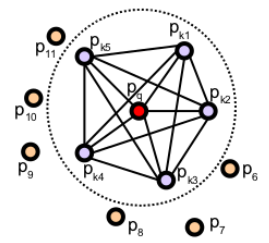
\includegraphics[width=7cm]{image/PFH.png}
    \caption{Exemple de voisinage pris en compte dans le calcul de la courbure du descripteur PFH}
    \label{fig:pfhNeighborhood}
  \end{center}
\end{figure}
Le descripteur PFH calculé en un point correspond à la relation que ce point a avec l'ensemble des points de son voisinage. Cette relation
est la différence des normals entre deux points. Chaque classe de l'histogramme est composé de l'ensemble des points du voisinage dont 
la relation avec le point centrale est similaire.
%FPFH
%SHOT
\subsubsection{Apprentissage automatique}
%svm
%random forest
\subsubsection{Bag of word}

\subsection{Positionnement de modèle}
%moment d'inertie pour la position des membres
%PCA
